%!TEX root = ../talk.tex
\chapter{Overview and Comparison of P2P File Synchronization and Storage Solutions}
\markboth{Overview and Comparison of P2P File Synchronization and Storage Solutions}{}
\chaptauthors{Josua Fr\"ohlich, Simon Ruesch}

\Kurzfassung{
Today, file synchronization and storage are demanded more than ever. The average user owns multiple devices that are continuously connected to the internet and works on the device which is the most practical for his current situation. As a consequence, users require their files to be up-to-date at all times regardless on which device the user wants to access the files. A second aspect is that there is an ever increasing demand for systems which allow file sharing between users, so multiple people can work on the same files independently, whether at the same time or not. Traditional cloud-based file storage and synchronization systems cover these requirements but also come with drawbacks, mainly with regards to security and availability in case of server faults or attacks. To address these drawbacks, P2P file storage and synchronization systems have been developed.
This seminar report gives an overview over the current available P2P file storage systems and categorizes them according to their different aspects. A set of criteria was determined to compare the systems.
The findings of the report show that P2P systems can be an improvement over cloud-based systems regarding security and fault-tolerance but they exhibit problems in other areas like availability and trust. The examined systems all specialize in a certain aspect and, as a trade-off, are worse in others.
}

\newpage

% the table of contents
\minitoc

\newpage

\section{Introduction and Problem Statement}
Today, file synchronization and storage are demanded more than ever. The average user owns multiple devices that are continuously connected to the internet and works on the device which is the most practical for his current situation. As a consequence, users require their files to be up-to-date at all times regardless on which device the user wants to access the files. A second aspect is that there is an ever increasing demand for systems which allow file sharing between users, so that multiple people can work on the same files independently, whether at the same time or not.

In general, existing file synchronization and storage systems can be categorized into two groups: Client-Server-based distributed file storage systems (also sometimes referred to as Cloud storage systems) and Peer-to-Peer file storage systems. The focus of this report lies on Peer-to-Peer file storage systems.

This seminar report provides an overview over the current available P2P file storage systems and compare them based on a set of chosen comparison criteria described in Chapter \ref{subsec:criteria}. In Chapter \ref{sec:background}, the term Peer-to-Peer systems is explained and the historical development of different file storage systems is presented. Chapter \ref{sec:approach} explains the reasons for the decisions made for the choice of systems to compare and also for the criteria according to which the systems were compared with each other. The following four P2P systems have been chosen and will be described in Chapter \ref{comparisons} according to the chosen criteria: Storj, AeroFS, Hive2Hive and BitTorrent Sync. Those P2P systems are also compared to Dropbox, a typical example for a cloud-based file storage system. Furthermore, the findings will be summarized by comparing the advantages and drawbacks of these systems.

\section{Background}
\label{sec:background}
This section gives a short basic overview over the most important topics concerning P2P systems, file storage, and the special requirements of P2P file storage systems compared to those of traditional and distributed file storage. Also, the most common drawbacks of these older systems compared to P2P systems will be shown.

\subsection{File Storage}
The Free Dictionary defines file storage as follows:
\begin{quote}
A generic term for warehousing electronic files. It may refer to local storage in a PC or tablet or remote storage on the Internet. The primary storage devices are hard drives and solid state drives. \cite{thefreedictionary}
\end{quote}
First of all, an overview of the different approaches to file storage and some historical aspects will be given. Three different generations of file storage can be classified. From here on, the term distributed file storage (DFS) signifies file storage that is not managed by only one system that is constricted to one geographic location. The term \textit{cloud} is used as a metaphorical synonym for DFS. The following content refers to Wu \ref{p2p:introduction_storage_systems}.

The first class of file storage is \textit{Client-Server file storage}, also called \textbf{1st generation DFS}, which is a system where the cloud consists of one or multiple huge file server storing all the files of multiple clients on the same network. The main problem of such a system is that the file server itself acts as a \textit{single point of failure}, as illustrated in Figure \ref{1st_gen_dfs}.

\textit{Distributed file systems}, known as \textbf{2nd generation DFS}, not to be confused with distributed file storage, show some similarities to the traditional system, except files being stored on a cluster of servers, so each server stores parts of the original files. Often, RAID (Redundant Array of Independent Disks) is used to avoid storage medium failure and enhance data throughput. These systems are known to be symmetric and scalable. Scalable is an indicator for how easy it is to add endpoints to a system. Figure \ref{2nd_gen_dfs} shows a scheme of a distributed file system.

The \textbf{3rd generation DFS}, also called \textit{P2P file storage systems}, in general do not have a clear structure and separation between clients and servers. Each peer, which means each device connected to the network that is able to store or access data on that network, is connected to other peers, see Figure \ref{3rd_gen_dfs}. The whole system is self-organizing, autonomous and heterogeneous. Heterogeneity in the sense of what systems are within such a network and what bandwidth rate is available, meaning it does not matter whether a peer is a powerful server on broadband or a mobile device on it's mobile network. Autonomy and self-organization is the basic principle and indicator for P2P systems and describes the process of how other peers can be discovered and how the network sets itself up. Peers can give access, read and or write to other peers to specific files and folders, and as long as the peers providing the data are connected to the network, the files are accessible.
	
\begin{figure}
	\centering
	\begin{minipage}{.33\textwidth}
		\centering
		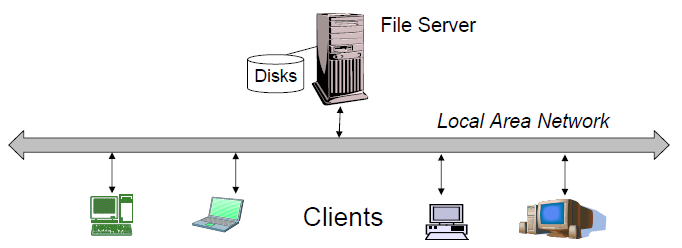
\includegraphics[scale=0.175]{Talk5/1st_gen_dfs.PNG}
		\caption[myfakelabel]{1st gen. DFS\footnotemark[1]{}}
		\label{1st_gen_dfs}
	\end{minipage}%
	\begin{minipage}{.33\textwidth}
		\centering
		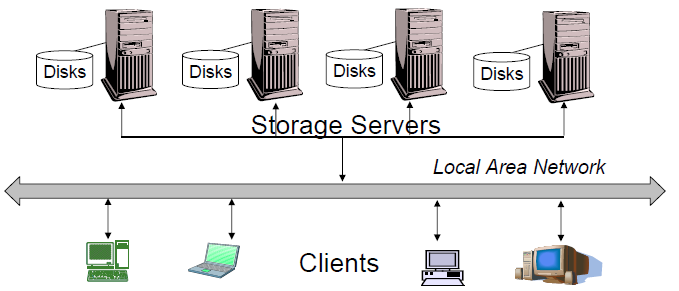
\includegraphics[scale=0.175]{Talk5/2nd_gen_dfs.PNG}
		\caption[myfakelabel]{2nd gen. DFS}
		\label{2nd_gen_dfs}
	\end{minipage}
	\begin{minipage}{.33\textwidth}
		\centering
		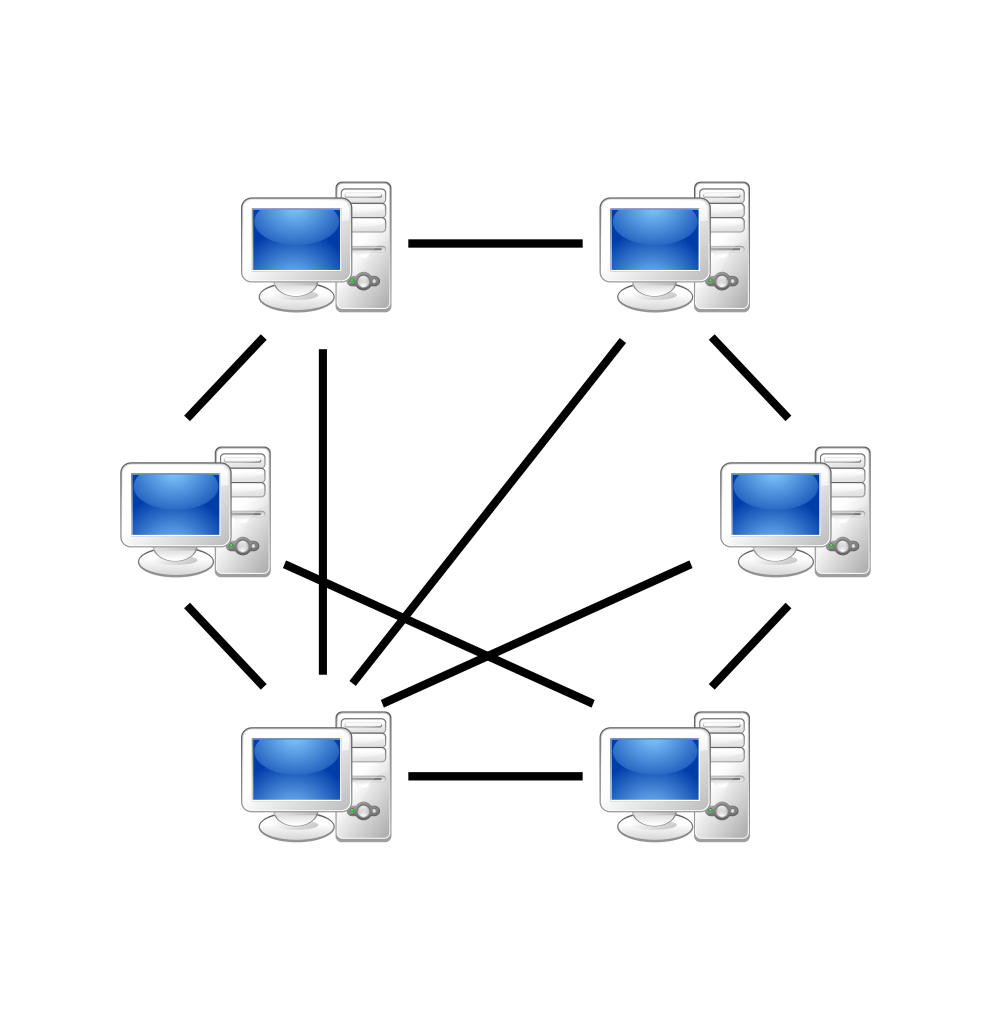
\includegraphics[scale=0.175]{Talk5/3rd_gen_dfs.PNG}
		\caption[myfakelabel]{3rd gen. DFS\footnotemark[1]{}}
		\label{3rd_gen_dfs}
	\end{minipage}
\end{figure}
\footnotetext[1]{Peer-to-peer; http://en.wikipedia.org/wiki/Peer\_to\_peer, online accessed at April, 2015.}

As each approach of distributed file storage has its benefits, there is no system without drawbacks or constraints. In the following chapter, Chapter \ref{subsec:peer-to-peer} different peering solutions and their known advantages and drawbacks are discussed.

\subsection{Peer-to-Peer}
\label{subsec:peer-to-peer}
In this section, a description of the main principles and goals of P2P systems will be given. First, a definition of P2P systems is presented. Second, it is explained what types of structures for peer connections exist, and thirdly, a summary of the well known advantages and drawbacks of P2P systems compared to traditional cloud storage is shown.
\begin{quote}
A distributed network architecture may be called a Peer-to-Peer (P-to-P, P2P,...) network, if the participants share a part of their own hardware resources (processing power, storage capacity, network link capacity, printers,...). These shared resources are necessary to provide the Service and content offered by the network (e.g. file sharing or shared workspaces for collaboration). They are accessible by other peers directly, without passing intermediary entities. The participants of such a network are thus resource (Service and content) providers as well as resource (Service and content) requestors (Servent-concept). \cite{p2p:definition}
\end{quote}
The goal behind P2P systems is to move away from the traditional client-server architecture with the goal to also avoid it's drawbacks. Instead of having one machine acting as a server, only answering requests by clients when these clients send those requests, in P2P, the roles of the client and server are combined into one machine. Peers then can form a network of peers, i.e., a P2P network.

There are some well-known advantages and disadvantages in P2P systems. In traditional distributed file storage, the server can become the single point of failure and RAID networks are expensive and sophisticated to maintain whereas P2P networks do not have to deal with these problems. P2P systems are scalable and sophisticated in fault tolerance which is hard to achieve for traditional distributed file storage systems. However, P2P systems are quite difficult to manage and good security is hard to achieve. However, these tasks can be more easily handled by a single peer, acting as a central authority, similar to traditional distributed file storage systems \cite{openp2p:p2p_introduction}.

Generally, P2P networks can be classified into four different types. In most cases, it is not possible to clearly associate a system to only one of these four classes because most systems do not provide such a clear structure or use multiple approaches. Nonetheless, usually one approach is more prevalent than others \cite{openp2p:p2p_introduction}.
\begin{enumerate}
	\item \textbf{Centralized P2P} as indicated in Figure \ref{centralized_p2p} shows similarities to the classical client-server model where even though peers communicate directly with each other, they also use some capabilities of a central server. A well-known service as an example for centralized P2P is Napster in which a central peer serves as a file directories. AeroFS, discussed in Chapter \ref{subsec:Aerofs} uses a similar approach.

	\item \textbf{Hybrid P2P} provides so called \textit{super peers} to find other peers and resources. Peers communicate to these super peers until the resource is found, at which point the peers can communicate directly with each other. A well-known service of this class is Skype. Figure \ref{hybrid_p2p} illustrates the hybrid approach.
	
	\item \textbf{Pure P2P} systems, also known as \textit{unstructured P2P} systems, are systems in which all peers communicate directly without any server or super peer and act as relays to find demanded resources. BitTorrent Sync and Storj, both systems that will be discussed in detail in Chapter \ref{subsec:bittorrent} and \ref{subsec:storj} are systems which use a pure P2P approach as shown in Figure \ref{pure_p2p}.
	
	\item \textbf{Structured P2P} systems, as shown in Figure \ref{structured_p2p}, are similar to pure P2P, however, the peers are organized in a specific structure, e.g. a tree or a Distributed Hash Table (DHT), which is used to improve peer and resource detection. A DHT, much like a normal hash table is a data structure that stores key-value pairs. However, in the DHT, the key-value pairs are distributed among peers, where each peer is responsible for storing the key-value pairs of a certain key range.
\end{enumerate}

\begin{figure}
	\begin{minipage}{.5\linewidth}
		\centering
		
\includegraphics[scale=0.2]{Talk5/centralized_p2p.PNG}
		\caption{Centralized P2P}
		\label{centralized_p2p}
	\end{minipage}%
	\begin{minipage}{.5\linewidth}
		\centering
		
\includegraphics[scale=0.2]{Talk5/hybrid_p2p.PNG}
		\caption{Hybrid P2P}
		\label{hybrid_p2p}
	\end{minipage}\par\medskip
	\begin{minipage}{.5\linewidth}
		\centering
		
\includegraphics[scale=0.2]{Talk5/pure_p2p.PNG}
		\caption{Pure (unstructured) P2P}
		\label{pure_p2p}
	\end{minipage}%
	\begin{minipage}{.5\linewidth}
		\centering
		
\includegraphics[scale=0.2]{Talk5/structured_p2p.PNG}
		\caption{Structured P2P}
		\label{structured_p2p}
	\end{minipage}%
\end{figure}

P2P networks often lack of having enough peers who are continuously connected to the network \ref{storj:PDF}.

\subsection{Problems of Synchronization and Sharing Services}
File synchronization and storage has to deal with several problems. Depending on the type of file storage and synchronization that is used, some problems are easy to address and some are very hard to fully cover. In traditional file storage, the main problem is the server itself which becomes a single point of failure and is vulnerable to targeted attacks, e.g., DDOS (distributed denial of service) attacks. Also, private data on these large, external data centers is often not encrypted or, if it is, the keys are stored on the same server, as will be shown in Chapter \ref{subsec:dropbox}. Additionally, users do not have control over who can access their private data and he or she is bound to the respective pricing and terms of the service. Such systems also often lack version control and conflict management \cite{hive2hive}.

Also manageability and trust are topics P2P solutions have to address. Depending on the type of P2P network structure used, e.g., manageability gets more complicated as it is for pure P2P and availability is downscaled in centralized P2P where the server again becomes a single point of failure. Concerning trust, it has been proven that powerful and well secured servers have been successfully undermined. It is just a logic implication that for peers, which represent normal household computational devices, manipulation must be much simpler \ref{openp2p:p2p_introduction}.

\section{Approach}
\label{sec:approach}
In this section, the reasons for the choice of systems are provided. Additionally, the criteria chosen to compare the different file storage systems are listed and stated in Section \ref{subsec:criteria}.

\subsection{Selection Criteria}
During research, so many P2P systems where discovered that making a selection of a subset to compare was inevitable. The selection criteria were:
\begin{enumerate}
\item \textbf{Availability and maturity} -- \textit{Is the system currently available and are the concepts developed and implemented and not just ideas?}\\
A good documentation or papers of the systems was required to be able to cover as many comparison criteria of Section \ref{subsec:criteria} as possible.

\item \textbf{Academic or commercial release} -- \textit{Was or is the system being developed for academical purposes or is the system available commercially?}\\
A mixture of academical and commercial systems gives a more diverse overview since only few systems could be chosen.

\item \textbf{Importance in future} -- \textit{Does the system show features which indicate that it might play an important role in the future?}\\
Admittingly hard to estimate, this criteria was chosen to select systems that are expected to be around for the next few years.
\end{enumerate}

\subsection{Comparison Criteria}
\label{subsec:criteria}
The decision of comparsion criteria was made to fit the most important aspects a prospective user considers before making the decision of which file storage system to use. The following criteria were chosen for comparison, and a justification for each choice is given.

\begin{enumerate}[(a)]
\item \textbf{Peer Connection} -- \textit{How are peers connected, where is user data stored, how do users communicate and what messages do they exchange?}\\
This criteria describes the technical aspects of the P2P system. As described in Section \ref{sec:background} there are many different forms of how peers can be connected in P2P networks. It is also important for users to know how and where their data is physically stored in the network. Some users may be cautious with storing their personal data on the machine of a stranger, even if the data is divided into chunks and encrypted. This aspect also deals with how peers can share data with each other and which communication possibilities exist. 

\item \textbf{Encryption} -- \textit{Is the communication between peers and the files stored encrypted and with which algorithm?}\\
Users tend to give great importance to the fact that their personal data can only be read by authorized peers. Therefore, a strong encryption mechanism is almost mandatory. This criteria analyzes if and how the users' files and their communications with other peers are encrypted.

\item \textbf{Trust and Integrity} -- \textit{How is trust established between peers? How are files and communications protected against fraudulent users and attacks?}\\
A peer must be able to check if other peers are who they claim to be allowing a peer the decision to trust another peer. Furthermore, this criteria looks at how users can verify the integrity of their files, i.e., if there haven't been any malicious changes to them.

\item \textbf{Payment Scheme} -- \textit{Is the system free or paid? Who gets paid how much under which circumstances?}\\
A user is more likely to use a system the cheaper it is. However, some systems also allow users to earn money by using the system, e.g., by offering up their excess storage space.

\item \textbf{Fairness} -- \textit{How is the workload distributed in the system especially considering the heterogeneous hardware used by the peers?}\\
A system has to balance the workload of file storage equally among the peers, such that not a single peer is storing all files of all peers. It is undesirable for a peer to take part in a system where it has a large workload compared to the benefit gained. Also, an uneven distribution can lead to the problem of single points of failure.

\item \textbf{Fault-tolerance and Availability} -- \textit{How does the system guarantee that files are available to the users at all time?}\\
The system should handle network failures and prevent data loss when a peer unexpectedly drops from the network. Also, users tend to be impatient and do not want to wait for hours until they can access their data.

\item \textbf{Distribution of Service} -- \textit{Is the system only a library or a dedicated software client?}\\
This aspect determines the ease of use of the system, but also if a expert user can build his or her own application on top of the provided system.

\item \textbf{Source code availability} -- \textit{Is the system open-source or closed source?}\\
This aspect is most relevant to application developers but might also be of interest for conventional users. If a system is open source, an application developer can make changes to the program code and may also contribute to future releases of the system. However, this can also be detrimental. Programmers may be able to change certain parts of their application which in turn may bypass security and fairness concepts normally applied in the system. Closed source code can also be disadvantageous. If the source code is not accessible, users have to trust the developer that the security algorithms are properly implemented and that their data is only accessible to authorized parties. With open source code, an adept user can at all times verify the quality of the security scheme.

\item \textbf{User base} -- \textit{How many users does the system currently have? Is the system intended for businesses or private users?}\\
Firstly, the amount of users already using the system are an indication of the quality of the system to prospective users. Network effects exist which make it more useful for users to use a system which is already widely established instead of one which is only used by few people. Additionally, an open source system with many active users and developers are more secure than one with a smaller install base. However, a larger user base also makes the system a more desirable target of attacks by malicious users. Secondly, the feature set of a system can also be geared more towards business applications instead of private users. It is usually more prudent to choose a system that is more suitable to the goals of the user.

\item \textbf{Status} -- \textit{In what state is the system? Is it available for use, a scientific prototype or canceled?}\\
A system should be available for use or at least available in near future. Also digital aging of systems that are no longer officially supported has to be considered, since data storage is not meant to last only for a few months or years. Scientific prototypes are important to get to know what the current point of technology is able to achieve and thus have a possible view into the future where more systems with such approaches may be used.
\end{enumerate}

\section{Comparisons}
\label{comparisons}
In this section, we compare four exemplary P2P file storage systems according to the comparison criteria given in the preceding section. We also compare the P2P file storage to Dropbox, a popular distributed file storage system to find similarities and differences. The systems analyzed are, in order, Dropbox, Storj, Hive2Hive, BitTorrent Sync and finally AeroFS. At the end, the findings are highlighted in a table comparing the file storage systems with each other.

\subsection{Dropbox}
\label{subsec:dropbox}
As a comparison to the chosen P2P systems, the well-known file hosting service Dropbox that was founded in 2007 will be used as representation for classical cloud storage solutions and measured according to the same criteria. Both cloud storage and file synchronization are possible with this service.

\textbf{Peer Connection:} Dropbox does not use any P2P technology but rather a client-server system. The data is stored in the Amazon S3 cloud. An authorization system is provided and users can give other users access to their data with either read-only or read and write permission. Folders and files can be shared by link or by username (registration required).

\textbf{Encryption:} The stored data is encrypted with AES-256 and upload to and download from the servers is encrypted. The main critique point is that Dropbox stores the decryption keys on their servers thus administrators have insight into the data.

\textbf{Trust \& Integrity:} Dropbox does not provide a mechanism to establish trust. Rather, it is the users' responsibility to only share the file links with people they trust.

\textbf{Payment Scheme:} Dropbox employs a Freemium model where base use is free and more storage can be aquired through a paid subscription.
\begin{enumerate}[(a)]
	\item Dropbox Basic - free - 2 GB
	\item Dropbox Pro - 10 Euro / month - 1 TB
	\item Dropbox for Business - 12 Euro / month - unlimited
\end{enumerate}

\textbf{Fairness:} The fairness criteria is not applicable for Dropbox, since all files are stored on the Dropbox servers.

\textbf{Fault-tolerance and Availability:} Dropbox servers act as single point of failure.

\textbf{Distribution of Service:} Dropbox can be accessed through their website, but a desktop GUI application also exists.

\textbf{Source code availability:} Closed source.

\textbf{User base:} Around 300 mio. (29.05.2014)\cite{dropbox:userbase}.

\textbf{Status:} Available for usage.

\subsection{Storj}
\label{subsec:storj}
Storj (pronounced storage) is a decentralized and blockchain-based P2P cloud storage system with it's major concern for security and efficiency. Having been launched in July 2014, it includes a P2P payment system service similar to Bitcoin \cite{storj:blog:what_is_storj}. Storj mainly consists of two applications, namely DriveShare (also called Driveminer) and Metadisk. The former uses unused hard drive space of users and the latter is a web-service used for file storage and sharing. Storj suggests that the average user has a lot of unused hard drive space and for many systems a user pays for a specific amount of space even if he or she doesn't use it at all. Storj further claims a Storj user is only obliged to pay for his used space and thus it will be much cheaper than any other available cloud storage. The following sections refer to Wilkinson \textit{Storj A Peer-to-Peer Cloud Storage Network} \cite{storj:PDF}.

\textbf{Peer Connection:} There are no centralized servers but information of where other shards of a specific file are located is stored in the Storj blockchain. A shard is a fixed size piece of a file, multiples of which are distributed to other peers. In the blockchain itself no files but only meta-data (file hashes) for file lookup are stored. A blockchain is very hard to manipulate as every peer gets a copy of it. Peer discovery is done by an advertisement system whose functionality is not explained in precision. Storj remains an unstructured P2P system using the blockchain as reference for file discovery.

\textbf{Encryption:} Before encryption and distribution, files are split into shards. These shards, a multiple of 8 or 32 Bit-sized file chunks, are added a deterministic salt, then uniquely encrypted and distributed over the network. A farmer, which means a hard drive space providing peer, does not get a whole copy of a file (all necessary shards to compose the original file) but the shards are distributed to multiple farmers. Per default there are at least three redundant copies of a shard available at all times. For enhanced security and for sensitive or important data, it is also possible to combine shards, e.g. with garbage data or data of other clients. The \textit{proof of redundancy} claims that if a node goes offline a copy of all it's shards is made and the shards moved to another node. In addition, a user can choose with which algorithm his or her files are encrypted.

\textbf{Trust and Integrity} Storj uses a so-called \textit{pseudo-reputation system}, that is like advertisements in peer discovery, to get data quality and type. Evaluations are made either by tracking or directly from the network to detect and qualify reputable peers. A peer is reputable if it is marked as trustworthy by the algorithm. Storj uses a recommendation system for peers to improve the algorithm.

The \textit{proof of storage} via \textit{Merkle audits}, or audits through \textit{hash challenge} ensure whether a farmer is able to proof that he holds a specific file, or more precise, a specific shard and that the shard has not been modified. The Merkle tree used for the Merkle audit is a hash tree where every non-leaf node is labeled with the hash of the labels of its children nodes, so to find out whether a child has been modified, it is sufficient to check if the parent node has a correct hash.

Storj uses different so called \textit{heartbeats} to check whether a file is correctly divided into shards and stored. Shards are furthermore split into pieces and checked for fulfillment of the security requirements and modification detection through heartbeats as shown in Figure \ref{storj_heartbeat}. A \textit{full heartbeat} means the whole shard integrity is checked, but this is shown to be very I/O inefficient whereas \textit{cycle heartbeats} need \textsl{n} heartbeats to generate a full heartbeat. Deterministically generated reads on a shard using a root seed is the third variant for those audits (\textit{cycle heartbeat}), but Storj uses a mixed methodology to improve efficiency.

	\begin{figure}[ht]
		\begin{center}
		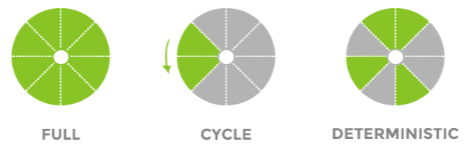
\includegraphics[scale=0.8]{Talk5/storj_heartbeat.PNG}
		\end{center}
		\caption{Heartbeat shard audit \cite{storj:PDF}}
		\label{storj_heartbeat}
	\end{figure}

But what happens if a malicious farmer knows the decryption key of a specific file? According to Wilkinson the malicious farmer won't be able to complete the audits (heartbeats) for all shards since he or she isn't assigned to all of them. In addition, this leads to the \textit{prove of redundancy} of particular shards which means that each copy of a shard is unique.

\textbf{Payment scheme:} With DriveShare, users, the so called farmers, can lease their unused available hard drive space and get paid for this service in Storjcoin X (SJCX), which is based on Bitcoin. SJCX rewards depend on the current crowdsale phase and are between 38'500 and 32'480 SJCX per Bitcoin \cite{storj:crowdsale}. Users of Metadisk will pay bitcoin (BTC) for these hard drive space to be able to share their files.

\textbf{Fairness:} Storj has no central devices and through the \textit{proof of redundancy} it is guaranteed that the files are evenly distributed. Also prices can vary on the base of bandwidth and location of the peer and type of hardware provided.

\textbf{Fault-tolerance and Availability:} By default there are three copies of a shard accessible at all times which means a shard gets copied to another node if a node goes offline. The user can request more copies in exchange for money. In this way, if a node fails an audit or is unreachable, the \textit{network replication process} is initiated and thus the network is able to restore itself. Storj illustrates the basic principle behind a blockchain as follows:

\begin{quotation}
To use a basic analogy, it is easy to steal a cookie from a cookie jar in a secluded area, but it is hard to do so when the jar is instead located in the middle of a public square, being observed by thousands of people. \cite{storj:PDF}
\end{quotation}

\textbf{Distribution of Service:} As mentioned above Storj consists of two applications; DriveShare and Metadisk.

\textbf{Source code availability:} Both applications (and even more Storj applications) are fully open-source \cite{storj:github}.

\textbf{User base:} There is no official up-to-date data and the system is currently in beta-phase. The forum of Storj has over one thousand members \cite{storj:forum} and it can be assumed that there are more Storj users in total. In June 2014 Storj had more than 3'000 users \cite{storj:crowdsale}.

\textbf{Status:} Being in beta phase, Storj is already available for use. There are three different test groups; A, B and C each with different conditions in terms of a reward system, requirements and the starting date. The official launch and every change in beta phase is planned when a specific amount of SJCX in total has been achieved \cite {storj:earlyaccess}.

\subsection{Hive2Hive}
Hive2Hive \cite{hive2hive}, formerly known as Box2Box, is an open source P2P file sharing and synchronization library that started out as part of a course challenge task project and was further improved in a graduate student's project at the Communication Systems Group at the University of Zurich \cite{hive2hive:about}. It is built on top of the TomP2P library (an open source, DHT-based key-value store) which was also developed at the Communication Systems Group \cite{tomp2p}.

\textbf{Peer Connection}
A structured P2P network is used. Each peer is assigned an ID which signifies for which key range the peer is responsible for storage. For each piece of data that is to be stored in the DHT, an ID is generated that shows at which peer the file is stored. Those IDs are generated with a hash function that hashes a certain piece of information that is only known by authorized peers. That means that only peers who have the correct permission have that piece of information and therefore can access that data. The central piece of data for a user is his or her user profile, which is stored with a hash of the password and pin of the user. Those are generated when first registering to the system and have to be kept secret from all other peers. The user profile contains the encryption keys of the user and also the file tree, which is a replica of the local file system of the user which holds the files that are stored on his or her system. The file tree consists of file indexes which represent individual files, each containing the ID of a metadata object. These metadata objects are separately stored in the DHT and contain the IDs of the file chunks. Before storage, files are divided into chunks and a random ID is generated for each chunk and stored in the metadata file of that file. A file chunk is stored at the peer with the ID closest to the hashed ID of the chunk.

\textbf{Encryption}
Hive2Hive uses a hybrid encryption mechanism for files stored in the DHT. AES-256 is used for symmetrical encryption and RSA with 2048 bit keys is used for asymmetrical encryption. Messages between users are encrypted asymmetrically with a different set of RSA keys. The keys are stored in the user profile stored in the DHT, which is only accessible by the user which the profile belongs to.

\textbf{Trust \& Integrity}
There are two types of file access permission that can be given to other peers, read access and read/write access. Peers without any of those permissions cannot access a file. File chunks are signed with an MD5 hash to guarantee integrity. Peers have to verify the identity of the peers that they want to share files with themselves.

\textbf{Payment Scheme}
Hive2Hive is open source and is like most open source software free of charge to use.

\textbf{Fairness}
Since IDs for file chunks are generated randomly, the file chunks are distributed equally between all peers in the long run. However, there is no mechanism in place that prevents peers from storing an extraordinary amount of files.

\textbf{Fault-tolerance and Availability}
By default, file chunks are replicated three times but higher amounts can be configured.

\textbf{Distribution of Service}
Hive2Hive itself is a library that provides the functionality of file sharing and synchronization. However, an end-user GUI application called Peerwasp \cite{peerwasp} is currently in development that uses Hive2Hive as a basis.

\textbf{Source code availability}
The source code of Hive2Hive, TomP2P as well as Peerwasp is freely available on Github \cite{hive2hive:github}, \cite{tomp2p:github}, \cite{peerwasp:github}. 

\textbf{User base}
Since Hive2Hive is distributed as a library and the developers do not provide an official number, the user base is hard to estimate.

\textbf{Status}
A library with active development.

\subsection{BitTorrent Sync}
\label{subsec:bittorrent}
Sync is a P2P file synchronization system developed by BitTorrent, the company that also developed the famous BitTorrent P2P protocol for file sharing. Development for Sync started in 2013 and Sync officially left beta in March 2015.

\textbf{Peer Connection}
In Sync, users do not enter a large static network per se. Rather, connections between peers are established as soon as they start sharing folders with each other. To share a folder, the user can generate a link to it through the software. This link has to be distributed out of band, e.g., through email to the person to share the folder with. The link has to be kept a secret between the peers, since it contains the encryption key of the folder. Also, the link contains a so-called shareID which is unique for each folder and is used to advertise who can access a given folder in the Sync system. There are four different possibilities of peer discovery, i.e., finding out the IP address of a peer: Firstly, if the IP address of the peer is known to the user, it can be entered manually. Secondly, a DHT is in place that can be queried for the shareID and returns the IP address of the authorized peers. Thirdly, there are tracker servers that store a shareID / authorized peers IP address mapping table. Lastly, peers can advertise their shared folders in the LAN through multicast. Any user is free to decide which combination of peer discovery he or she wants to use.

\textbf{Encryption}
Sync uses AES-128 encryption for files while they are in transit. Additionally, the X.509 protocol and SSL are used to encrypt communication between peers.

\textbf{Trust \& Integrity}
The trust in Sync depends on the discretion of how the link to the shared folders is distributed. Users have to be careful that they only provide the link to people that they know are trustworthy. However, Sync also allows users to give their peers either only read access or full read/write access to folders.

\textbf{Payment Scheme}
Sync is available as a free version, but there is also a paid version for 39.99 euros per year that allows users, among other benefits, to share an unlimited number of folders.

\textbf{Fairness}
The fairness criteria is not applicable to Sync, since files are only shared between a few select peers and they then receive a full copy of the file, therefore all peers store all shared files.

\textbf{Fault-tolerance and Availability}
Since the files are only synchronized between a few trusted peers, one of those peers has to be online for a new peer to enter the synchronization and access the files. The system is fault-tolerant in terms of peer discovery as described above.

\textbf{Distribution of Service}
Sync is available as a desktop application as well as an application for mobile phones.

\textbf{Source code availability}
BitTorrent Sync is currently closed source.

\textbf{User base}
The latest known number from 2014 claims a user base of 10 million users.

\textbf{Status}
As of March 2015, Sync is fully released to the public.

\subsection{AeroFS}

\label{subsec:Aerofs}
AeroFS is a dedicated software client from Air Computing that provides basic P2P solutions but also some advanced functionality concerning security and encryption, error and data loss prevention and intends to offer the service at a low cost. AeroFS is mainly targeted towards business users and companies who need a secure file backup and synchronization service \cite{aerofs}. AeroFS in addition claims to be the 'P2P version' of Dropbox.

\textbf{Peer Connection:} AeroFS uses a centralized P2P network but lets the user choose how this will be managed. Air Computing offers two different cloud options and as an Add-on, the Team Server:

\begin{enumerate}
\item \textbf{Private Cloud}: Provides private Web Administration, the AeroFS Appliance which is a lightweight virtual machine to manage registration and authentication of users and private Certificate Authority (CA) to manage the AeroFS public key infrastructure (PKI) for client applications.
\item \textbf{Hybrid Cloud}: Supplies a centrally managed file sharing platform for the employees; registration, authentication and user management is done outside the network by AeroFS.
\item \textbf{Team Server} (optional Add-on): Lightweight client to enable backup of files and 24/7 availability \cite{aerofs:cloud_types}. The Team Server itself has three different options:
	\begin{enumerate}[(a)]
	\item \textbf{Linked Storage}: Creates a read/write copy of organization's files on the Team Server. Files will still be browseable.
	\item \textbf{Block Storage}: Compresses and de-duplicates files for enlarged disk space. Files won't be browseable anymore.
	\item \textbf{S3 Storage}: Data shared by users of an organization is stored and backed up on Amazon servers compressed and de-duplicated. Files won't be browseable anymore \cite{aerofs:storage_types}.
	\end{enumerate}
\end{enumerate}

\textbf{Encryption:} An \textit{end-to-end encryption} solution is provided, files are encrypted before transaction using AES-256 with 2048-bit RSA and only the recipient is able to decrypt the data transfer \cite{aerofs:security}. The files for syncing are eventually stored unencrypted. Depending on the solution used, the AeroFS servers store only usernames, the hashes of the passwords and the names of all users authorized to access each folder (hybrid) \cite{aerofs:security_2}.

\textbf{Trust and Integrity} The amount of users for a AeroFS administrator account, typically a company, is of fixed size (but can grow). Also using the AeroFS Applicance as root certificate, no other footprint will be accepted by the clients \cite{aerofs:security}. AeroFS provides three different access permission:
\begin{enumerate}[(a)]
\item Owners (poject administrators): Can add and remove members to the shared folder.
\item Editors: Can create and modify content.
\item Viewers: Can only read content.
\end{enumerate}
A user can manage the AeroFS public key infrastructure (PKI) with his or her AeroFS Appliance as the root certificate authority (CA). The clients are configured to trust only this AeroFS Appliance which limits the trust footprint. AeroFS also provides an option to wipe data from stolen devices.

\textbf{Payment scheme:} The basic pricing plan (Team) is free up to a user-base of 30 \cite{aerofs:blog:30_users_free} and the business plan starts above 31 users and the billing is done according to the number of users; One user costs \$15, the highest number of users on the website is 1'000 users for \$15'000 per month \cite{aerofs:pricing}.

\textbf{Fault-tolerance and Availability:} Multiple users can work on the same file and conflicts are resolved by the users themselves by comparing the changes and thus resolve the conflicts. But the AeroFS Appliance and the AeroFS Servers act as single point of failure and no user will be able to register and authenticate anymore in case of failure.

\textbf{Fairness:} AeroFS provides a load balancer for the AeroFS Appliance which acts as a single API endpoint and securely forwards API requests to running Team Servers and desktop clients. This load balancer thus tries to distribute the workload evenly by maintaining the balance between service availability and data consistency. If a runs out of hard drive space, the versioning systems of the AeroFS Team Server keeps track of the oldest copies and deletes them \cite{aerofs:USTO.RE}. Fairness in the sense of P2P is not applicable or not relevant since a peering network only consists of known peers, e.g., within a company.

\textbf{Distribution of Service:} AeroFS offers a software client and the AeroFS Appliance for users and a admin dash panel for enhanced manageability.

\textbf{Source code availability:} AeroFS is currently closed source but there are some open-source projects on the AeroFS Github page.

\textbf{User base:} According to the webpage \cite{aerofs} there are currently around \textbf{50'000\textsc{+}} users.

\textbf{Status:} Available for use.

\subsection{Summary}
\label{subsec:summary}
% Some text that refers to the table
In Table \ref{table}, the findings of the comparison are summarized. The research has shown that there are many possible solutions for each of the chosen criteria, so that the chosen systems differ greatly especially in the criterias peer connection, trust and integrity, fault-tolerance and fairness. It is apparent that some criterias correlate, e.g., a system that has a paid variant typically also has a closed source code. As expected, Dropbox shows weaknesses in the criteria that were posited as weak points for the entire class of cloud-based file storage systems, i.e., trust and integrity and fault-tolerance. However, the P2P systems are not necessarily better in those aspects. Neither Hive2Hive nor BitTorrent Sync provide mechanisms for establishing trust between peers inside the system itself and AeroFS assumes that all users are trusted because its main focus is the deployment in a single company. However, P2P systems perform better with regards to fault-tolerance by either splitting files into redundant number of chunks and distributing them in the network or by storing a copy of the entire file on each synchronized device.

\begin{sidewaystable}
	\centering
	\caption{Comparison of four different P2P Systems in comparison to Dropbox}
	\label{table}
		\begin{tabular}{ | *{6}{ p{2.5cm} |} }
			\hline
			& Dropbox & Storj & AeroFS & Hive2Hive & Sync \\ \hline
			Peer Connection & None & Unstructured & Centralized & Structured & Unstructured / Structured / Centralized \\ \hline
			Encryption & Files encrypted, key stored on server & End-End, user defined algorithm & End-End, AES-256 with 2048-bit RSA & Hybrid Encryption for files, Asymmetric for messages & AES-128 for files in transit, X.509 and SSL \\ \hline
			Trust and Integrity & File links out of band & Audits (Heartbeats) & AeroFS Appliance / AeroFS Server & Signed messages / Data & Folder links distributed out of band \\ \hline
			Payment & Free / Paid & Paid & Free / Paid & Free & Free / Paid \\ \hline
			Fault-Tolerance & Single point of failure & Replication of shards & Copy of each file on each synced device / Backup on Team Server & File chunks replicated & Copy of each file on each synced device \\ \hline
			Fairness & Not applicable & Even & Load balancer (Team Server only) & Even & Not applicable \\ \hline
			Distribution & Desktop App / Web & Desktop App / Web & Desktop App & Library & Desktop App \\ \hline
			Source Code & Closed & Open & Closed & Open & Closed \\ \hline
			User Base & >300 Mio & ~3k & ~50k & Unknown & >10 Mio \\ \hline
			Status & Available & Beta & Available & Active development & Available \\ \hline
		\end{tabular}
\end{sidewaystable}

\section{Conclusions}

The results of the research show that P2P developers have found many different solutions to face the problems that come up when developing and constructing such a system. Thus to simplify implementation there is almost always a specialization of the software for a specific use. To benefit from one aspect of a P2P network it might be inevitable to afford drawbacks and constraints in another aspect. Concretely one could imagine a slider going from e.g. left, fault-tolerance to right, Availability and every developer have to decide where to place his slider between because it is not possible to have them both on 100 percent. Publisher often care about a specific application area, e.g., business use or file synchronization and thus the 'sliders' have to be set as appropriate as possible for every system. Further, a clear separation between file synchronization and file storage need to be made. P2P systems are able to do both but depending on the choice of specialization, doing both might no always be as easy.

Trade-off

As a conclusion of the facts described above P2P systems as well as client-server models do not solve all problems and requirements of file storage and synchronization. One has to always live with some constraints or privacy issues, e.g., the gap between trusting a (well-known) storage provider versus a (anonymous) peer. P2P does not automatically mean that the single point of failure problem is solved, many P2P systems are not really better than traditional cloud storage systems in this aspect. P2P systems are also vulnerable to certain types of attacks that traditional client-server models are not, e.g., Sybil attacks.

Future work:
- other criteria (ease of use, performance)
- other systems

\begin{thebibliography}{99}

	\bibitem {p2p:definition}
		R. Schollmeier:
		\emph{A definition of peer-to-peer networking for the classification of peer-to-peer architectures and applications;}
		Peer-to-Peer Computing, 2001. Proceedings. First International Conference,
		August 2001,
		pp.101,102,
		\url{http://ieeexplore.ieee.org/stamp/stamp.jsp?tp=&arnumber=990434&isnumber=21356}.

	\bibitem {aerofs}
		\emph{AeroFS}
		\url{https://www.aerofs.com/},
		online accessed at March, 2015.

	\bibitem {aerofs:security_2}
		\emph{AeroFS: Das bessere Dropbox? - Golem.de;}
		\url{http://www.golem.de/news/aerofs-das-bessere-dropbox-1304-98485.html},
		online accessed at April, 2015.

	\bibitem {aerofs:blog:30_users_free}
		Y. Sagalov:
		\emph{AeroFS is now free up to 30 users;}
		\url{https://www.aerofs.com/blog/aerofs-is-now-free-up-to-30-users/},
		online accessed at April, 2015.
		
	\bibitem {bitcoin}
		S. Nakamoto:
		\emph{Bitcoin: A Peer-to-Peer Electronic Cash System;}
		\url{https://bitcoin.org/bitcoin.pdf},
		online accessed at April, 2015.

	\bibitem {bittorrentsync-2}
		J. Farina, M. Scanlon, M. Kechadi:
		\emph{BitTorrent Sync: First Impressions and Digital Forensic Implications;}
		Proceedings of the First Annual DFRWS Europe,
		\url{http://ac.els-cdn.com/S1742287614000152/1-s2.0-S1742287614000152-main.pdf?_tid=10ddb6e2-ce69-11e4-9019-00000aacb35d&acdnat=1426791318_6677afbe19d521d323605261c1d19809},
		Volume 11, Supplement 1, Pages S77\textendash S86, Volume 11, May, 2014.

	\bibitem {box2box}
		A. Lareida, T. Bocek, S. Golaszewski, C. L\"uthold, M. Weber:
		\emph{Box2Box - A P2P-based File-Sharing and Synchronization Application;}
		\url{http://www.csg.uzh.ch/csg/live/teaching/FS13/p2p/challenge/P2P2013DP_017.pdf},
		online accessed at April, 2014.

	\bibitem {dropbox:userbase}
		\emph{Dropbox Reaches 300M Users;}
		\url{http://thenextweb.com/insider/2014/05/29/dropbox-reaches-300m-users-adding-100m-users-just-six-months/},
		online accessed at April, 2015.

	\bibitem {aerofs:cloud_types}
		\emph{Enterprise Solution - Deployment Options, AeroFS;}
		\url{https://www.aerofs.com/features/deployment-options/},
		online accessed at April, 2015.

	\bibitem {thefreedictionary}
		\emph{File Storage Definition;}
		\url{http://encyclopedia2.thefreedictionary.com/file+storage},
		online accessed at April, 2015.

	\bibitem {aerofs:peering_scheme_2}
		\emph{Flexible Storage for the Enterprise;}
		\url{https://www.aerofs.com/features/flexible-storage/},
		online accessed at April, 2015.

	\bibitem {hive2hive:about}
		\emph{Hive2Hive: About Us;}
		\url{https://github.com/Hive2Hive/Hive2Hive/wiki/About-Us},
		online accessed at March, 2015.

	\bibitem {hive2hive:github}
		\emph{Hive2Hive: Java library for secure, distributed, P2P-based file synchronization and sharing;}
		\url{https://github.com/Hive2Hive},
		online accessed at March, 2015.
	(https://github.com/tomp2p/TomP2P) (https://github.com/PeerWasp/PeerWasp)

	\bibitem {hive2hive}
		\emph{Hive2Hive: Open-Source Library for P2P-based File Synchronization and Sharing;}
		\url{http://hive2hive.com/},
		online accessed at March, 2015.

	\bibitem {metadisk}
		S. Wilkinson, J. Lowry:
		\emph{Metadisk: Blockchain-based decentralized file storage application;}
		\url{http://metadisk.org/metadisk.pdf},
		online accessed at April, 2014.
		
	\bibitem {p2pfswu}
		C. Wu:
		\emph{Peer-to-Peer Networks;}
		\url{http://www.csie.nuk.edu.tw/~wuch/course/csf641/csf641-04-storage.pdf},
		online accessed at March, 2015.

	\bibitem {p2pfskangasharju}
		J. Kangasharju:
		\emph{Peer-to-Peer Networks Chapter 4: Peer-to-Peer Storage;}
		\url{http://www.cs.helsinki.fi/u/jakangas/Teaching/P2P/P2P-04-Storage.pdf},
		online accessed at March, 2015.

	\bibitem {peerwasp}
		\emph{Peerwasp, P2P File Synchronization and Sharing Solution based on Hive2Hive and TomP2P}
		\url{http://www.peerwasp.com/},
		online accessed at April, 2015.

	\bibitem {peerwasp:github}
		\emph{Peerwasp, P2P File Synchronization and Sharing Solution based on Hive2Hive and TomP2P}
		\url{https://github.com/PeerWasp/PeerWasp},
		online accessed at April, 2015.

	\bibitem {aerofs:pricing}
		\emph{Pricing, AeroFS;}
		\url{https://www.aerofs.com/pricing/},
		online accessed at April, 2015.

	\bibitem {aerofs:security}
		\emph{Security, AeroFS;}
		\url{https://www.aerofs.com/security/},
		online accessed at April, 2015.
		
	\bibitem {aerofs:peering_scheme}
		\emph{Security Share and Transfer Large Files, Enterprise Solution, Aerofs;}
		\url{https://www.aerofs.com/solutions/transfer-large-files/},
		online accessed at April, 2015.
		
	\bibitem {storj:PDF}
		S. Wilkinson:
		\emph{Storj A Peer-to-Peer Cloud Storage Network;}
		\url{http://storj.io/storj.pdf/},
		online accessed at April, 2014.
		
	\bibitem {storj:crowdsale}
		\emph{Storj Deck - Decentralized Cloud;}
		\url{http://storj.io/Deck.pdf},
		online accessed at April, 2015.

	\bibitem {storj:earlyaccess}
		\emph{Storj - Early Access;}
		\url{http://storj.io/earlyaccess.html},
		online accessed at April, 2015.
		
	\bibitem {storj:github}
		\emph{Storj Labs;}
		\url{https://github.com/Storj/},
		online accessed at March, 2015.
		
	\bibitem {storj:deck}
		\emph{Storj - The Crowdsale;}
		\url{http://storj.io/crowdsale.html},
		online accessed at March, 2015.
		
	\bibitem {storj:forum}
		\emph{Storjtalk;}
		\url{https://storjtalk.org/},
		online accessed at April, 2015.
		
	\bibitem {bittorrentsync}
		\emph{Sync;}
		\url{https://www.getsync.com/},
		online accessed at March, 2015.

	\bibitem {p2p:introduction_storage_systems}
		Prof. Chun-Hsin Wu:
		\emph{P2P Storage Systems;}
		\url{http://www.csie.nuk.edu.tw/~wuch/course/csf641/csf641-04-storage.pdf},
		online accessed at Mai, 2015.
		
	\bibitem {p2p-introduction:tomp2p}
		\emph{TomP2P: A P2P-based high performance key-value pair storage library;}
		\url{http://tomp2p.net/doc/p2p/},
		online accessed at April, 2015.		

	\bibitem {tomp2p}
		\emph{TomP2P, a P2P-based high performance key-value pair storage library;}
		\url{http://tomp2p.net},
		online accessed at April, 2015.

	\bibitem {tomp2p:github}
		\emph{TomP2P, a P2P-based high performance key-value pair storage library}
		\url{https://github.com/tomp2p/TomP2P},
		online accessed at April, 2015.

	\bibitem {openp2p:p2p_introduction}
		\emph{Distributed Systems Topologies: Part 2 - O'Reilly Media;}
		\url{hhttp://www.openp2p.com/pub/a/p2p/2002/01/08/p2p_topologies_pt2.html},
		online accessed at Mai, 2015.

	\bibitem {aerofs:USTO.RE}
		Dur\~ao et al:
		\emph{USTO.RE: A Private Cloud Storage Software System;}
		\url{http://www.researchgate.net/profile/Vinicius_Garcia/publication/262284124_USTO.RE_a_private_cloud_storage_software_system/links/5457a3f30cf2cf51648219ed.pdf},
		online accessed at April, 2015.

	\bibitem {storj:blog:what_is_storj}
		\emph{What ist Storj?;}
		\url{http://blog.storj.io/post/87251450053/what-is-storj},
		online accessed March, 2015.

	\bibitem {aerofs:storage_types}
		\emph{What Storage Types Can I Use With The AeroFS Team Server? - AeroFS Support;}
		\url{https://support.aerofs.com/hc/en-us/articles/203434524},
		online accessed at April, 2015.

\end{thebibliography}